\chapter{Continuity: Functions that Preserve Closeness}

\section{From Sequences to Functions}

\begin{intuition}
We've studied sequences: discrete points approaching a limit.

Now we study \textbf{continuous functions}: functions where ``nearby inputs produce nearby outputs.''

\textbf{Informal idea}: A function $f$ is continuous if you can draw its graph without lifting your pen.

\textbf{Rigorous idea}: $f$ is continuous at $x$ if $f(x_n) \to f(x)$ whenever $x_n \to x$.

This chapter makes continuity precise and proves its fundamental properties.
\end{intuition}

\begin{historicalnote}
\textbf{The Evolution of Continuity}

\textbf{Ancient Mathematics (300 BCE - 1600 CE)}:
\begin{itemize}
    \item Greeks used continuous curves geometrically (circles, conics)
    \item No formal definition---continuity was intuitive
    \item Archimedes: Method of exhaustion assumed continuity implicitly
\end{itemize}

\textbf{Early Calculus (1650-1800)}:
\begin{itemize}
    \item Newton, Leibniz: Used continuous functions freely
    \item Euler: ``A continuous function is one whose equation is given by a single analytic expression''
    \item \textbf{Problem}: What about piecewise functions? No rigorous definition
\end{itemize}

\textbf{19th Century Rigor}:
\begin{itemize}
    \item \textbf{Bolzano (1817)}: First rigorous definition using sequences
    \item \textbf{Cauchy (1821)}: ``$f$ is continuous if infinitely small changes in $x$ produce infinitely small changes in $f(x)$'' (still vague)
    \item \textbf{Weierstrass (1860s)}: The modern $\epsilon$-$\delta$ definition
    \item \textbf{Key insight}: Replace vague ``infinitely small'' with precise quantifiers
\end{itemize}

\textbf{Impact}:
\begin{itemize}
    \item Allowed rigorous proofs of Intermediate Value Theorem, Extreme Value Theorem
    \item Revealed surprising phenomena: continuous but nowhere differentiable functions
    \item Foundation for topology (continuous functions between topological spaces)
\end{itemize}

The $\epsilon$-$\delta$ definition is one of the great achievements of 19th-century mathematics.
\end{historicalnote}

\section{Continuity at a Point}

\begin{definition}[Continuity at a Point (Sequential)]
Let $f: D \to \mathbb{R}$ where $D \subseteq \mathbb{R}$, and let $c \in D$.

The function $f$ is \textbf{continuous at $c$} if:

For every sequence $(x_n)$ in $D$ with $x_n \to c$, we have $f(x_n) \to f(c)$.

\textbf{In symbols}:
\[\forall (x_n) \subseteq D: x_n \to c \implies f(x_n) \to f(c)\]
\end{definition}

\begin{keyidea}
\textbf{Sequential continuity}: If inputs approach $c$, outputs approach $f(c)$.

This means: The limit of $f$ at $c$ equals the value of $f$ at $c$.

Equivalently: You can ``pass the limit through the function'':
\[\lim_{n \to \infty} f(x_n) = f\left(\lim_{n \to \infty} x_n\right)\]
\end{keyidea}

\begin{example}[Continuous Function]
Let $f(x) = x^2$. Prove $f$ is continuous at $c = 2$.

\textbf{Proof}: Let $(x_n)$ be any sequence with $x_n \to 2$.

We need to show $f(x_n) = x_n^2 \to 4 = f(2)$.

By algebra of limits:
\[\lim_{n \to \infty} x_n^2 = \left(\lim_{n \to \infty} x_n\right)^2 = 2^2 = 4\]

Therefore $f(x_n) \to f(2)$, so $f$ is continuous at $2$. $\checkmark$

(This argument works for any $c$, so $f(x) = x^2$ is continuous everywhere.)
\end{example}

\begin{example}[Discontinuous Function]
Define $f: \mathbb{R} \to \mathbb{R}$ by:
\[f(x) = \begin{cases}
0 & \text{if } x \neq 0 \\
1 & \text{if } x = 0
\end{cases}\]

\textbf{Claim}: $f$ is not continuous at $c = 0$.

\textbf{Proof}: Consider the sequence $x_n = \frac{1}{n} \to 0$.

Then $f(x_n) = 0$ for all $n$ (since $x_n \neq 0$), so $f(x_n) \to 0$.

But $f(0) = 1 \neq 0$.

Therefore $f(x_n) \not\to f(0)$, so $f$ is not continuous at $0$. $\blacksquare$
\end{example}

\vspace{0.5cm}
\begin{center}
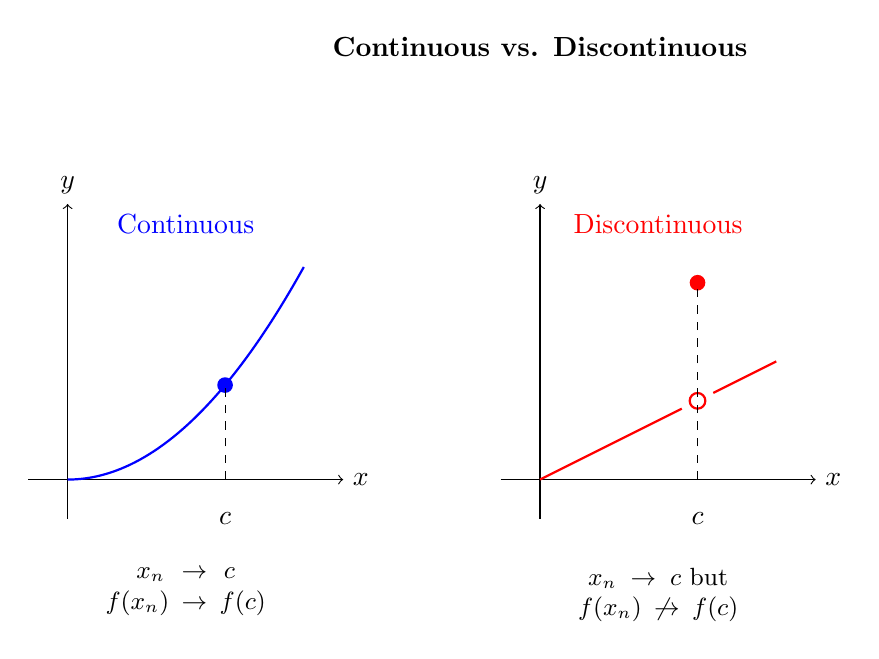
\begin{tikzpicture}[scale=1.0]
    \node at (6, 5.5) {\textbf{Continuous vs. Discontinuous}};
    
    % Continuous function
    \begin{scope}[xshift=0cm]
        \draw[->] (-0.5, 0) -- (3.5, 0) node[right] {$x$};
        \draw[->] (0, -0.5) -- (0, 3.5) node[above] {$y$};
        \draw[thick, blue, domain=0:3, samples=50] plot (\x, {0.3*\x*\x});
        \node[circle, fill=blue, inner sep=2pt] at (2, 1.2) {};
        \node[below] at (2, -0.3) {$c$};
        \draw[dashed] (2, 0) -- (2, 1.2);
        \node[above] at (1.5, 3) {\textcolor{blue}{Continuous}};
        \node[below, text width=3cm, align=center, font=\small] at (1.5, -1) {
            $x_n \to c$ \\
            $\implies f(x_n) \to f(c)$
        };
    \end{scope}
    
    % Discontinuous function
    \begin{scope}[xshift=6cm]
        \draw[->] (-0.5, 0) -- (3.5, 0) node[right] {$x$};
        \draw[->] (0, -0.5) -- (0, 3.5) node[above] {$y$};
        \draw[thick, red, domain=0:1.8] plot (\x, {0.5*\x});
        \draw[thick, red, domain=2.2:3] plot (\x, {0.5*\x});
        \node[circle, fill=white, draw=red, thick, inner sep=2pt] at (2, 1) {};
        \node[circle, fill=red, inner sep=2pt] at (2, 2.5) {};
        \node[below] at (2, -0.3) {$c$};
        \draw[dashed] (2, 0) -- (2, 2.5);
        \node[above] at (1.5, 3) {\textcolor{red}{Discontinuous}};
        \node[below, text width=3cm, align=center, font=\small] at (1.5, -1) {
            $x_n \to c$ but \\
            $f(x_n) \not\to f(c)$
        };
    \end{scope}
\end{tikzpicture}
\end{center}
\vspace{0.5cm}

\section{The $\epsilon$-$\delta$ Definition}

\begin{intuition}
The sequential definition is intuitive, but sometimes we need a definition that doesn't mention sequences.

Weierstrass's $\epsilon$-$\delta$ definition captures the same idea directly:

\textit{``For any desired closeness $\epsilon$ of outputs, there exists a required closeness $\delta$ of inputs.''}
\end{intuition}

\begin{definition}[Continuity at a Point ($\epsilon$-$\delta$)]
Let $f: D \to \mathbb{R}$ where $D \subseteq \mathbb{R}$, and let $c \in D$.

The function $f$ is \textbf{continuous at $c$} if:

\[\forall \epsilon > 0, \exists \delta > 0 \text{ such that } \forall x \in D: |x - c| < \delta \implies |f(x) - f(c)| < \epsilon\]

\textbf{In words}: For any $\epsilon$-neighborhood around $f(c)$, we can find a $\delta$-neighborhood around $c$ whose image lies entirely within the $\epsilon$-neighborhood.
\end{definition}

\begin{keyidea}
\textbf{The $\epsilon$-$\delta$ game}:

\textbf{Challenger}: Gives you $\epsilon > 0$ (tolerance for output)

\textbf{You}: Must find $\delta > 0$ such that whenever $|x - c| < \delta$, we have $|f(x) - f(c)| < \epsilon$

If you can always win, $f$ is continuous at $c$.

\textbf{Geometric interpretation}:
\begin{center}
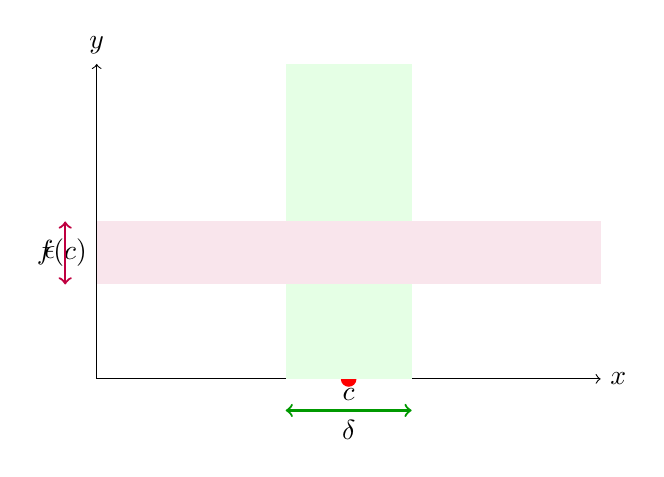
\begin{tikzpicture}[scale=0.8]
    \draw[->] (0, 0) -- (8, 0) node[right] {$x$};
    \draw[->] (0, 0) -- (0, 5) node[above] {$y$};
    
    % Function curve
    \draw[thick, blue, domain=0.5:7.5, samples=50] plot (\x, {2 + 0.3*sin(100*\x)});
    
    % Point c and f(c)
    \node[circle, fill=red, inner sep=2pt] (c) at (4, 0) {};
    \node[below] at (c) {$c$};
    \node[circle, fill=red, inner sep=2pt] (fc) at (4, 2) {};
    \node[left] at (0, 2) {$f(c)$};
    
    % Delta interval
    \draw[<->, thick, green!60!black] (3, -0.5) -- (5, -0.5);
    \node[below] at (4, -0.5) {$\delta$};
    
    % Epsilon interval
    \draw[<->, thick, purple] (-0.5, 1.5) -- (-0.5, 2.5);
    \node[left] at (-0.5, 2) {$\epsilon$};
    
    % Shaded regions
    \fill[green!10] (3, 0) rectangle (5, 5);
    \fill[purple!10] (0, 1.5) rectangle (8, 2.5);
\end{tikzpicture}
\end{center}

The green region (width $2\delta$) maps into the purple region (height $2\epsilon$).
\end{keyidea}

\begin{theorem}[Equivalence of Definitions]
The sequential definition and $\epsilon$-$\delta$ definition of continuity are equivalent.
\end{theorem}

\begin{proof}
\textbf{($\epsilon$-$\delta$ $\Rightarrow$ Sequential)}:

Assume $f$ satisfies the $\epsilon$-$\delta$ condition at $c$. Let $(x_n)$ be a sequence in $D$ with $x_n \to c$.

We show $f(x_n) \to f(c)$.

Let $\epsilon > 0$ be given. By $\epsilon$-$\delta$ continuity, there exists $\delta > 0$ such that:
\[|x - c| < \delta \implies |f(x) - f(c)| < \epsilon\]

Since $x_n \to c$, there exists $N$ such that for all $n \geq N$: $|x_n - c| < \delta$.

Therefore for $n \geq N$: $|f(x_n) - f(c)| < \epsilon$.

Thus $f(x_n) \to f(c)$. $\checkmark$

\textbf{(Sequential $\Rightarrow$ $\epsilon$-$\delta$)}:

Assume $f$ satisfies the sequential condition at $c$. We prove $\epsilon$-$\delta$ by contradiction.

Suppose $f$ does not satisfy $\epsilon$-$\delta$. Then there exists $\epsilon > 0$ such that for all $\delta > 0$, there exists $x$ with:
\[|x - c| < \delta \quad \text{but} \quad |f(x) - f(c)| \geq \epsilon\]

For each $n \in \mathbb{N}$, choose $\delta = \frac{1}{n}$. Then there exists $x_n$ such that:
\[|x_n - c| < \frac{1}{n} \quad \text{but} \quad |f(x_n) - f(c)| \geq \epsilon\]

The sequence $(x_n)$ satisfies $x_n \to c$ (since $|x_n - c| < \frac{1}{n} \to 0$).

By sequential continuity, $f(x_n) \to f(c)$.

But $|f(x_n) - f(c)| \geq \epsilon$ for all $n$, contradicting $f(x_n) \to f(c)$.

Therefore the $\epsilon$-$\delta$ condition must hold. $\blacksquare$
\end{proof}

\begin{example}[Using $\epsilon$-$\delta$ to Prove Continuity]
Prove $f(x) = 3x + 2$ is continuous at $c = 1$ using $\epsilon$-$\delta$.

\textbf{Proof}: Let $\epsilon > 0$ be given. We need to find $\delta > 0$ such that:
\[|x - 1| < \delta \implies |f(x) - f(1)| < \epsilon\]

Note that $f(1) = 3(1) + 2 = 5$.

\begin{align*}
|f(x) - f(1)| &= |(3x + 2) - 5| \\
&= |3x - 3| \\
&= 3|x - 1|
\end{align*}

We want $3|x - 1| < \epsilon$, so $|x - 1| < \frac{\epsilon}{3}$.

\textbf{Choose} $\delta = \frac{\epsilon}{3}$.

Then for $|x - 1| < \delta$:
\[|f(x) - f(1)| = 3|x - 1| < 3\delta = 3 \cdot \frac{\epsilon}{3} = \epsilon\]

Therefore $f$ is continuous at $c = 1$. $\blacksquare$

(This argument works at any $c$, so $f(x) = 3x + 2$ is continuous everywhere.)
\end{example}

\section{Continuous Functions}

\begin{definition}[Continuous on a Set]
A function $f: D \to \mathbb{R}$ is \textbf{continuous on $D$} (or simply \textbf{continuous}) if $f$ is continuous at every point $c \in D$.
\end{definition}

\begin{theorem}[Algebra of Continuous Functions]
If $f$ and $g$ are continuous at $c$, then:
\begin{enumerate}
    \item $f + g$ is continuous at $c$
    \item $f - g$ is continuous at $c$
    \item $f \cdot g$ is continuous at $c$
    \item $\frac{f}{g}$ is continuous at $c$ (if $g(c) \neq 0$)
    \item $cf$ is continuous at $c$ for any constant $c \in \mathbb{R}$
\end{enumerate}
\end{theorem}

\begin{proof}[Proof of Sum Rule]
Let $(x_n)$ be a sequence with $x_n \to c$.

Since $f$ is continuous at $c$: $f(x_n) \to f(c)$.

Since $g$ is continuous at $c$: $g(x_n) \to g(c)$.

By algebra of limits:
\[(f + g)(x_n) = f(x_n) + g(x_n) \to f(c) + g(c) = (f + g)(c)\]

Therefore $f + g$ is continuous at $c$. $\blacksquare$

The other rules follow similarly.
\end{proof}

\begin{example}[Polynomial Functions]
Every polynomial $p(x) = a_n x^n + a_{n-1} x^{n-1} + \cdots + a_1 x + a_0$ is continuous on $\mathbb{R}$.

\textbf{Proof}: 
\begin{itemize}
    \item Constant functions are continuous (trivial)
    \item $f(x) = x$ is continuous (easy $\epsilon$-$\delta$ proof with $\delta = \epsilon$)
    \item $x^k$ is continuous (by product rule, since $x^k = x \cdot x \cdots x$)
    \item $a_k x^k$ is continuous (by scalar multiplication)
    \item $p(x)$ is continuous (by sum rule)
\end{itemize}
$\blacksquare$
\end{example}

\begin{example}[Rational Functions]
Every rational function $r(x) = \frac{p(x)}{q(x)}$ is continuous on its domain (where $q(x) \neq 0$).

\textbf{Proof}: By quotient rule, since polynomials are continuous. $\blacksquare$
\end{example}

\begin{theorem}[Composition of Continuous Functions]
If $f: D \to \mathbb{R}$ is continuous at $c$ and $g: E \to \mathbb{R}$ is continuous at $f(c)$ (with $f(D) \subseteq E$), then $g \circ f$ is continuous at $c$.
\end{theorem}

\begin{proof}
Let $(x_n)$ be a sequence in $D$ with $x_n \to c$.

Since $f$ is continuous at $c$: $f(x_n) \to f(c)$.

Let $y_n = f(x_n)$. Then $(y_n)$ is a sequence in $E$ with $y_n \to f(c)$.

Since $g$ is continuous at $f(c)$: $g(y_n) \to g(f(c))$.

Therefore:
\[(g \circ f)(x_n) = g(f(x_n)) = g(y_n) \to g(f(c)) = (g \circ f)(c)\]

Thus $g \circ f$ is continuous at $c$. $\blacksquare$
\end{proof}

\begin{example}
$h(x) = \sin(x^2 + 3x)$ is continuous on $\mathbb{R}$.

\textbf{Proof}: 
\begin{itemize}
    \item $f(x) = x^2 + 3x$ is continuous (polynomial)
    \item $g(y) = \sin(y)$ is continuous (proven using trigonometric identities and $\epsilon$-$\delta$)
    \item $h = g \circ f$ is continuous (composition rule)
\end{itemize}
$\blacksquare$
\end{example}

\section{The Intermediate Value Theorem}

\begin{intuition}
If you drive from elevation 100m to elevation 200m, you must pass through every elevation in between.

More generally: A continuous function on an interval takes all values between any two of its values.

This seemingly obvious statement requires completeness of $\mathbb{R}$ to prove!
\end{intuition}

\begin{theorem}[Intermediate Value Theorem (IVT)]\index{intermediate value theorem}\index{IVT}\index{continuity!intermediate value theorem}
Let $f: [a, b] \to \mathbb{R}$ be continuous on the closed interval $[a, b]$.

If $f(a) < k < f(b)$ (or $f(b) < k < f(a)$), then there exists $c \in (a, b)$ such that $f(c) = k$.

\textbf{In words}: A continuous function on a closed interval attains every value between its endpoints.
\end{theorem}

\begin{center}
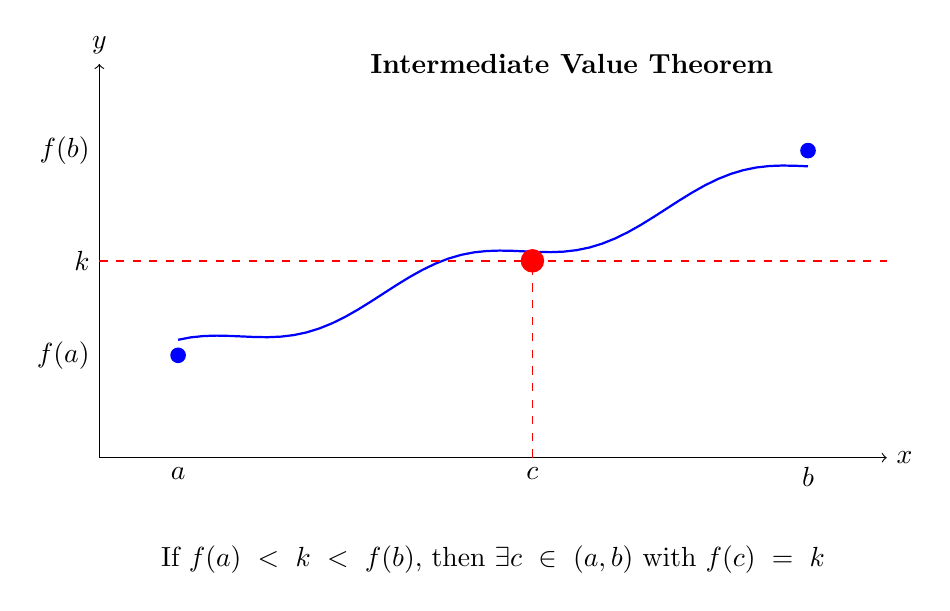
\begin{tikzpicture}[scale=1.0]
    \node at (6, 5) {\textbf{Intermediate Value Theorem}};
    
    \draw[->] (0, 0) -- (10, 0) node[right] {$x$};
    \draw[->] (0, 0) -- (0, 5) node[above] {$y$};
    
    % Continuous curve
    \draw[thick, blue, domain=1:9, samples=50] plot (\x, {1 + 0.3*\x + 0.2*sin(100*\x)});
    
    % Points a and b
    \node[circle, fill=blue, inner sep=2pt] at (1, 1.3) {};
    \node[below] at (1, 0) {$a$};
    \node[left] at (0, 1.3) {$f(a)$};
    
    \node[circle, fill=blue, inner sep=2pt] at (9, 3.9) {};
    \node[below] at (9, 0) {$b$};
    \node[left] at (0, 3.9) {$f(b)$};
    
    % Horizontal line at k
    \draw[dashed, red, thick] (0, 2.5) -- (10, 2.5);
    \node[left] at (0, 2.5) {$k$};
    
    % Intersection point c
    \node[circle, fill=red, inner sep=3pt] at (5.5, 2.5) {};
    \node[below] at (5.5, 0) {$c$};
    \draw[dashed, red] (5.5, 0) -- (5.5, 2.5);
    
    \node[below, text width=10cm, align=center] at (5, -1) {
        If $f(a) < k < f(b)$, then $\exists c \in (a,b)$ with $f(c) = k$
    };
\end{tikzpicture}
\end{center}

\begin{proof}
Assume $f(a) < k < f(b)$ (the other case is similar).

Define:
\[S = \{x \in [a, b] : f(x) < k\}\]

\textbf{Properties of $S$}:
\begin{itemize}
    \item $S \neq \emptyset$ (since $a \in S$, as $f(a) < k$)
    \item $S$ is bounded above (by $b$)
\end{itemize}

By completeness, $c = \sup(S)$ exists.

We show $f(c) = k$.

\textbf{Claim 1}: $f(c) \leq k$.

\textit{Proof}: Suppose $f(c) > k$. Let $\epsilon = f(c) - k > 0$.

By continuity, there exists $\delta > 0$ such that $|x - c| < \delta \implies |f(x) - f(c)| < \epsilon$.

For $x \in (c - \delta, c + \delta)$:
\[f(x) > f(c) - \epsilon = f(c) - (f(c) - k) = k\]

This means $f(x) > k$ for all $x$ near $c$, so no element of $S$ is close to $c$, contradicting $c = \sup(S)$. $\checkmark$

\textbf{Claim 2}: $f(c) \geq k$.

\textit{Proof}: Suppose $f(c) < k$. Let $\epsilon = k - f(c) > 0$.

By continuity, there exists $\delta > 0$ such that $|x - c| < \delta \implies |f(x) - f(c)| < \epsilon$.

For $x \in (c, c + \delta)$:
\[f(x) < f(c) + \epsilon = f(c) + (k - f(c)) = k\]

This means $c + \frac{\delta}{2} \in S$, contradicting $c = \sup(S)$. $\checkmark$

Therefore $f(c) = k$. $\blacksquare$
\end{proof}

\begin{keyidea}
The IVT uses completeness crucially:
\begin{enumerate}
    \item We define $S = \{x : f(x) < k\}$
    \item We take $c = \sup(S)$ (this requires completeness!)
    \item We show $f(c) = k$ using continuity
\end{enumerate}

Without completeness (e.g., in $\mathbb{Q}$), the theorem fails.

\textbf{Counterexample in $\mathbb{Q}$}: $f(x) = x^2$ on $[1, 2]$ is continuous, and $f(1) = 1 < 2 < 4 = f(2)$, but there is no $c \in \mathbb{Q}$ with $f(c) = 2$ (since $\sqrt{2} \notin \mathbb{Q}$).
\end{keyidea}

\begin{example}[Root Finding]
Show that $x^3 - 3x + 1 = 0$ has a solution in $[0, 1]$.

\textbf{Proof}: Let $f(x) = x^3 - 3x + 1$.

$f$ is continuous (polynomial).

$f(0) = 1 > 0$ and $f(1) = 1 - 3 + 1 = -1 < 0$.

By IVT, there exists $c \in (0, 1)$ such that $f(c) = 0$. $\blacksquare$
\end{example}

\begin{example}[Fixed Point]
Every continuous function $f: [0, 1] \to [0, 1]$ has a fixed point (a point $c$ where $f(c) = c$).

\textbf{Proof}: Let $g(x) = f(x) - x$.

$g$ is continuous (difference of continuous functions).

$g(0) = f(0) - 0 = f(0) \geq 0$ (since $f(0) \in [0, 1]$).

$g(1) = f(1) - 1 \leq 0$ (since $f(1) \in [0, 1]$).

\textbf{Case 1}: If $g(0) = 0$, then $f(0) = 0$, so $c = 0$ is a fixed point.

\textbf{Case 2}: If $g(1) = 0$, then $f(1) = 1$, so $c = 1$ is a fixed point.

\textbf{Case 3}: If $g(0) > 0$ and $g(1) < 0$, then by IVT, there exists $c \in (0, 1)$ with $g(c) = 0$, so $f(c) = c$. $\blacksquare$
\end{example}

\section{The Extreme Value Theorem}

\begin{theorem}[Extreme Value Theorem (EVT)]\index{extreme value theorem}\index{EVT}\index{continuity!extreme value theorem}\index{compactness}
If $f: [a, b] \to \mathbb{R}$ is continuous on the closed bounded interval $[a, b]$, then $f$ attains its maximum and minimum.

That is, there exist $c, d \in [a, b]$ such that:
\[f(c) \leq f(x) \leq f(d) \quad \text{for all } x \in [a, b]\]
\end{theorem}

\begin{proof}[Proof of Maximum (Minimum is Similar)]
\textbf{Step 1: $f$ is bounded above}.

Suppose not. Then for each $n \in \mathbb{N}$, there exists $x_n \in [a, b]$ with $f(x_n) > n$.

The sequence $(x_n)$ is bounded (in $[a, b]$), so by Bolzano-Weierstrass, there exists a convergent subsequence $x_{n_k} \to c$ for some $c \in [a, b]$.

By continuity, $f(x_{n_k}) \to f(c)$.

But $f(x_{n_k}) > n_k \to \infty$, contradiction.

Therefore $f$ is bounded above. $\checkmark$

\textbf{Step 2: $f$ attains its supremum}.

Let $M = \sup\{f(x) : x \in [a, b]\}$ (exists by completeness and Step 1).

For each $n \in \mathbb{N}$, by definition of supremum, there exists $x_n \in [a, b]$ with:
\[f(x_n) > M - \frac{1}{n}\]

By Bolzano-Weierstrass, there exists a subsequence $x_{n_k} \to d$ for some $d \in [a, b]$.

By continuity, $f(x_{n_k}) \to f(d)$.

Since $M - \frac{1}{n_k} < f(x_{n_k}) \leq M$ and $\frac{1}{n_k} \to 0$, we have:
\[f(x_{n_k}) \to M\]

By uniqueness of limits, $f(d) = M$.

Therefore $f$ attains its maximum at $d$. $\blacksquare$
\end{proof}

\begin{center}
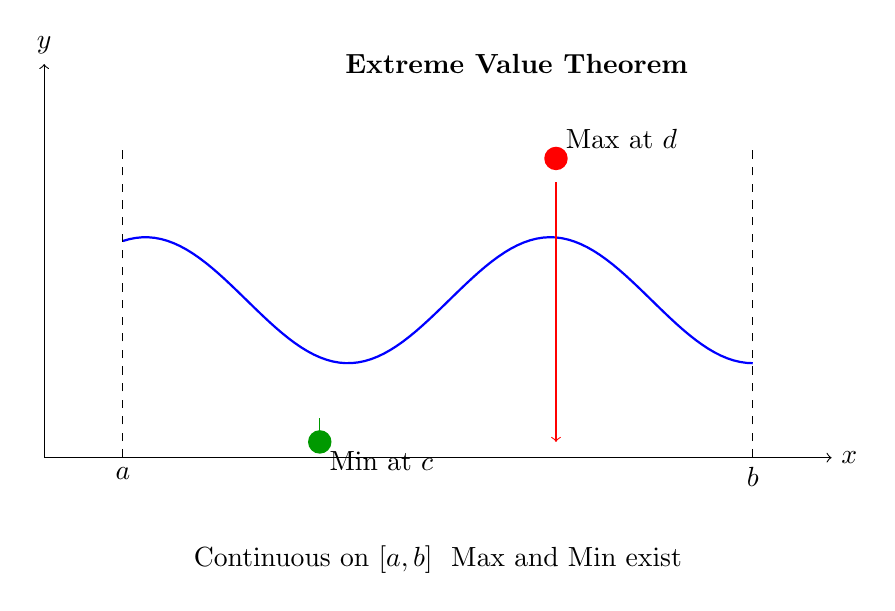
\begin{tikzpicture}[scale=1.0]
    \node at (6, 5) {\textbf{Extreme Value Theorem}};
    
    \draw[->] (0, 0) -- (10, 0) node[right] {$x$};
    \draw[->] (0, 0) -- (0, 5) node[above] {$y$};
    
    % Continuous curve with max and min
    \draw[thick, blue, domain=1:9, samples=100] plot (\x, {2 + 0.8*sin(70*\x)});
    
    % Interval endpoints
    \node[below] at (1, 0) {$a$};
    \node[below] at (9, 0) {$b$};
    \draw[dashed] (1, 0) -- (1, 4);
    \draw[dashed] (9, 0) -- (9, 4);
    
    % Maximum
    \node[circle, fill=red, inner sep=3pt] at (6.5, 3.8) {};
    \node[above right] at (6.5, 3.8) {Max at $d$};
    \draw[->, red] (6.5, 3.5) -- (6.5, 0.2);
    
    % Minimum
    \node[circle, fill=green!60!black, inner sep=3pt] at (3.5, 0.2) {};
    \node[below right] at (3.5, 0.2) {Min at $c$};
    \draw[->, green!60!black] (3.5, 0.5) -- (3.5, 0.2);
    
    \node[below, text width=10cm, align=center] at (5, -1) {
        Continuous on $[a,b]$ $\implies$ Max and Min exist
    };
\end{tikzpicture}
\end{center}

\begin{warning}
The EVT requires:
\begin{enumerate}
    \item \textbf{Continuity}: Without continuity, max/min may not exist
    \item \textbf{Closed interval}: On open intervals like $(a, b)$, max/min may not exist
    \item \textbf{Bounded interval}: On unbounded intervals like $[a, \infty)$, max/min may not exist
\end{enumerate}

\textbf{Counterexamples}:
\begin{itemize}
    \item $f(x) = x$ on $(0, 1)$: No max or min (open interval)
    \item $f(x) = \frac{1}{x}$ on $(0, 1]$: No max (not continuous at $0$)
    \item $f(x) = x$ on $[0, \infty)$: No max (unbounded interval)
\end{itemize}
\end{warning}

\begin{keyidea}
\textbf{Why EVT matters}:

Many optimization problems reduce to: ``Find the maximum/minimum of a continuous function on a closed bounded interval.''

EVT guarantees the solution exists---we just need to find it!

Typical strategy:
\begin{enumerate}
    \item Check continuity
    \item Check domain is closed and bounded
    \item Find critical points (where derivative is zero or undefined)
    \item Check endpoints
    \item Maximum is the largest value among these
\end{enumerate}
\end{keyidea}

\section{Uniform Continuity}

\begin{intuition}
A function is continuous if at each point $c$, we can find a suitable $\delta$ for any $\epsilon$.

But $\delta$ might depend on both $\epsilon$ \textit{and} the point $c$.

\textbf{Uniform continuity}: The same $\delta$ works for \textit{all} points simultaneously.
\end{intuition}

\begin{definition}[Uniform Continuity]\index{uniform continuity}\index{continuity!uniform}
A function $f: D \to \mathbb{R}$ is \textbf{uniformly continuous on $D$} if:

\[\forall \epsilon > 0, \exists \delta > 0 \text{ such that } \forall x, y \in D: |x - y| < \delta \implies |f(x) - f(y)| < \epsilon\]

\textbf{Key difference}: $\delta$ depends only on $\epsilon$, not on the specific points $x$ or $y$.
\end{definition}

\begin{example}[Uniformly Continuous Function]
$f(x) = 3x + 2$ on $\mathbb{R}$ is uniformly continuous.

\textbf{Proof}: Let $\epsilon > 0$ be given.

For any $x, y \in \mathbb{R}$:
\[|f(x) - f(y)| = |3x + 2 - 3y - 2| = 3|x - y|\]

We want $3|x - y| < \epsilon$, so $|x - y| < \frac{\epsilon}{3}$.

\textbf{Choose} $\delta = \frac{\epsilon}{3}$ (independent of $x, y$!).

Then $|x - y| < \delta \implies |f(x) - f(y)| = 3|x - y| < 3\delta = \epsilon$.

Therefore $f$ is uniformly continuous. $\blacksquare$
\end{example}

\begin{example}[Continuous but Not Uniformly Continuous]
$f(x) = x^2$ on $\mathbb{R}$ is continuous everywhere but \textit{not} uniformly continuous.

\textbf{Proof}: Suppose $f$ were uniformly continuous. Then for $\epsilon = 1$, there exists $\delta > 0$ such that:
\[|x - y| < \delta \implies |x^2 - y^2| < 1\]

Choose $x = n$ and $y = n + \frac{\delta}{2}$ for large $n$.

Then $|x - y| = \frac{\delta}{2} < \delta$, but:
\[|x^2 - y^2| = |n^2 - (n + \frac{\delta}{2})^2| = |−n\delta - \frac{\delta^2}{4}| \approx n\delta \to \infty\]

For sufficiently large $n$, this exceeds $1$, contradiction.

Therefore $f$ is not uniformly continuous on $\mathbb{R}$. $\blacksquare$
\end{example}

\begin{theorem}[Continuity on Compact Intervals]
If $f: [a, b] \to \mathbb{R}$ is continuous on the closed bounded interval $[a, b]$, then $f$ is uniformly continuous on $[a, b]$.
\end{theorem}

\begin{proof}[Proof Sketch]
Suppose $f$ is not uniformly continuous. Then there exists $\epsilon > 0$ such that for all $\delta > 0$, there exist $x, y$ with:
\[|x - y| < \delta \quad \text{but} \quad |f(x) - f(y)| \geq \epsilon\]

For each $n$, choose $\delta = \frac{1}{n}$, obtaining sequences $(x_n), (y_n)$ with:
\[|x_n - y_n| < \frac{1}{n} \quad \text{but} \quad |f(x_n) - f(y_n)| \geq \epsilon\]

By Bolzano-Weierstrass, $(x_n)$ has a convergent subsequence $x_{n_k} \to c \in [a, b]$.

Since $|x_{n_k} - y_{n_k}| < \frac{1}{n_k} \to 0$, we also have $y_{n_k} \to c$.

By continuity, $f(x_{n_k}) \to f(c)$ and $f(y_{n_k}) \to f(c)$.

Therefore $|f(x_{n_k}) - f(y_{n_k})| \to 0$, contradicting $|f(x_{n_k}) - f(y_{n_k})| \geq \epsilon$. $\blacksquare$
\end{proof}

\section{Looking Forward: Differentiation}

\begin{intuition}
Continuity means: Small changes in input produce small changes in output.

\textbf{Differentiability} strengthens this: Changes in output are \textit{linearly proportional} to changes in input (locally).

The derivative $f'(x)$ is the ``instantaneous rate of change''---the slope of the tangent line.

Next chapter: We'll define derivatives rigorously using limits and prove the fundamental theorems of calculus.
\end{intuition}

\begin{center}
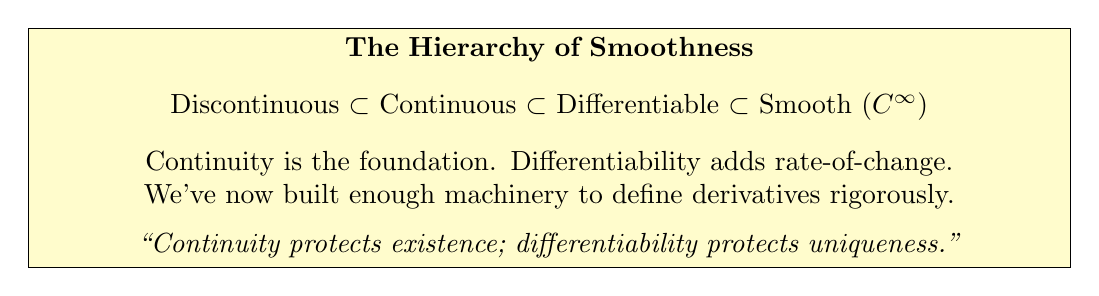
\begin{tikzpicture}[scale=1.0]
    \node[rectangle, draw, fill=yellow!20, text width=13cm, align=center] at (6.5, 0) {
    \textbf{The Hierarchy of Smoothness} \\[0.3cm]
    Discontinuous $\subset$ Continuous $\subset$ Differentiable $\subset$ Smooth ($C^\infty$) \\[0.3cm]
    Continuity is the foundation. Differentiability adds rate-of-change. \\
    We've now built enough machinery to define derivatives rigorously. \\[0.2cm]
    \textit{``Continuity protects existence; differentiability protects uniqueness.''} 
    };
\end{tikzpicture}
\end{center}
